% Results. Every number is generated into results.tex from saved artifacts
% by scripts/final_report.py; the prose below interprets, it does not
% transcribe. Locked-test numbers are added only after the single
% test-set evaluation.

\section{Results}
\label{sec:results}

\subsection{Numerical verification and the geometry correction}
\label{sec:res-verif}

The solver passes every test of Appendix~\ref{app:numerics}: first-order
convergence under grid and substep refinement, exact discrete flux balance,
preserved positivity, and reverse-mode gradients matching central
differences to nine or ten significant digits. At the operating resolution
the solver's own error is two orders of magnitude below the model--data
misfit, so no comparison drawn below is limited by numerics.

Two defects were found by verification and audit rather than by any training
or validation metric, and both are worth reporting because both were
invisible to the loss. The finite-volume cell volumes were inconsistent with
the face positions, which left the scheme stable and trainable but
non-convergent under refinement (Appendix~\ref{app:numerics}). More
seriously, the flux coordinate was inverted: MAST Level-2 stores poloidal
flux per radian, which is maximal on the magnetic axis, and the
normalisation assumed the opposite, placing $\rho = 1$ \emph{at} the
magnetic axis (Appendix~\ref{app:eq-rho}). Every profile was compressed into
$\rho \in [0.745, 1]$ non-monotonically, so the ``edge annulus'' that
carried all supervision was in fact the near-axis region.

The effect of correcting it is large and one-directional. Held-out profile
error falls from $\approx \SI{104}{eV}$ to $\SI{39}{eV}$--$\SI{41}{eV}$ in
the supervised annulus, a factor $2.6$; the best-checkpoint location moves
from step $150$--$250$ to $\approx 1850$; and, as \S\ref{sec:res-modelcomp}
shows, the ranking of the competing latent topologies reverses. We report
this sequence rather than only its endpoint because it is the clearest
evidence in this study that a fit which looks healthy by every training
diagnostic can still be fitted to the wrong part of the plasma.

\subsection{Held-out profile prediction}
\label{sec:res-profiles}

\begin{figure}[t]
  \centering
  
\includegraphics[width=0.66\linewidth]{figures/fig_fit}
  \caption{Free-running prediction on a held-out discharge (validation
  split). Dots: measured electron temperature at the three best-covered
  radii; line: model. Bottom: the inferred regime coordinate $\pH(t)$. The
  profile is integrated from its initial condition without measurement
  reset.}
  \label{fig:fit}
\end{figure}

On grouped-validation discharges the identified model reproduces the
measured edge temperature with a coverage-weighted mean absolute error of
$\SI{39}{eV}$--$\SI{41}{eV}$ ($28.5$--$29.8\%$ relative), consistently
across all three main configurations and all three seeds; the spread across
seeds within a configuration is below $\SI{2}{eV}$. This is a free-running
rollout: the profile is integrated from its initial condition with no
measurement reset, and only the measured edge boundary trace and the
measured density enter as time-varying inputs.

The residual source closure carries a substantial part of this accuracy.
Removing it entirely degrades the error to $\SI{58}{eV}$
(\S\ref{sec:res-ablations}), so the conservative diffusion operator alone
does not reproduce the observed edge evolution. This is expected for a
phenomenological temperature equation in which heating deposition,
radiation, and the neglected density and heat-capacity factors are all
absorbed into the residual term.

\subsection{Regime discrimination and calibration}
\label{sec:res-events}

Pooled over seeds, the median per-discharge AUC of the regime probability
against the weak labels is $0.912$ (95\% bootstrap CI $[0.909, 0.943]$) for
the extended-drive free-topology model, $0.942$ ($[0.900, 0.983]$) for the
constrained monostable model, and $0.920$ ($[0.909, 0.943]$) for the
injected-power drive. Roughly two thirds of held-out discharges exceed
AUC $0.9$ individually. Calibration behaves as described in
\S\ref{sec:ident-select}: raw expected calibration error is $0.14$--$0.33$
and falls to $0.036$--$0.095$ after validation-only Platt scaling, with
median Brier scores of $0.064$--$0.085$.

Event detection is a stricter test than discrimination, and the model is
markedly weaker on it. With one-to-one matching in a \SI{40}{ms} window,
L$\to$H recall reaches $0.40 \pm 0.03$ for the extended-drive free model and
$0.29$--$0.33$ for the others; matched events are located to a median
absolute timing error of a few tens of milliseconds. H$\to$L recall is
$0.00$ for every bistable fit and $0.10$ for the monostable ones. We regard
the low absolute recall as the principal limitation of the present model and
return to it in \S\ref{sec:discussion}.

\begin{figure}[t]
  \centering
  
\includegraphics[width=0.66\linewidth]{figures/fig_classification}
  \caption{Regime probability $\pH(t)$ (blue) for four held-out
  discharges; shaded bands mark the weakly labelled H segments. Shot
  numbers and split membership are given in each panel label.}
  \label{fig:classification}
\end{figure}

\begin{figure}[t]
  \centering
  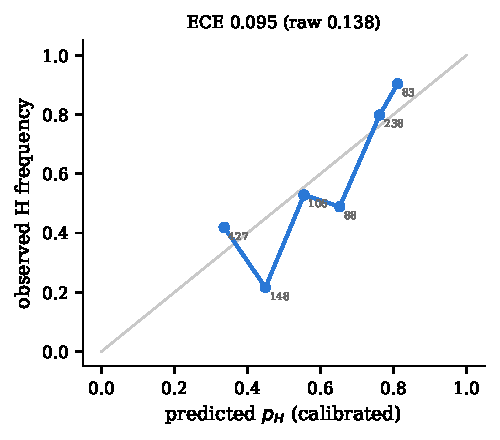
\includegraphics[width=0.52\linewidth]{figures/fig_reliability}
  \caption{Reliability of the regime probability on held-out discharges
  after validation-only Platt scaling; bin counts annotated. The
  uncalibrated expected calibration error is quoted for comparison in the
  panel title. Calibration is measured, not assumed.}
  \label{fig:reliability}
\end{figure}

\subsection{Do the data select a latent topology?}
\label{sec:res-modelcomp}

This is the question the study was designed to answer, and the answer is
negative. Table~\ref{tab:comparison} (generated from saved artifacts) reports the
three configurations at three seeds each under identical data, splits, solver, optimiser, stopping
rule, and parameter budget; only the named factor differs.

Two findings separate cleanly from seed noise, which is $\pm 0.001$--$0.013$
on these quantities.

\paragraph{The physics-directed drive extension is accepted.} Replacing the
injected-power drive $(P_{\mathrm{NBI}}, |I_p|, \bar n_e)$ with
$(P_{\mathrm{loss}}, |I_p|, \bar n_e, P_{\mathrm{rad}}, \kappa, \delta)$
improves held-out trajectory loss from $0.514 \pm 0.013$ to
$0.424 \pm 0.013$ and L$\to$H recall from $0.29 \pm 0.00$ to
$0.40 \pm 0.03$, at equal AUC. Both gaps are many seed-standard-deviations
wide. The covariates that help are precisely those that MAST threshold
studies identify as controlling: a loss-power rather than injected-power
measure of the drive, and the plasma shape.

\paragraph{The topology question is not decided by these data.} The free
model attains the better trajectory loss ($0.424 \pm 0.013$ against
$0.464 \pm 0.006$) and the better L$\to$H recall; the constrained monostable
model attains the better discrimination ($0.941 \pm 0.001$ against
$0.916 \pm 0.006$), the better calibration (Brier $0.064 \pm 0.002$ against
$0.081 \pm 0.005$), and the only non-zero back-transition recall. The
disagreement is systematic across seeds and runs in opposite directions on
different endpoints. That pattern --- consistent, reproducible, and
non-transitive --- is what ``the evidence does not decide'' looks like when
it is measured on several endpoints rather than one scalar.

The free fit does return a positive topology parameter reproducibly
($\beta = +0.303, +0.296, +0.295$ across seeds, a spread of $\pm 0.004$),
which under \eqref{eq:folds} implies a bistable vector field with folds at
$\dr_{\mathrm{f}}^{\pm} = \pm 0.06$. We report this as a property of the
fitted parameter set and explicitly not as evidence that the data require
folds, because a model forbidden from having folds describes the same
discharges at least as well.

\paragraph{Why bistability cannot capture the back-transitions.} The zero
H$\to$L recall of every bistable fit is structural rather than incidental.
Once the latent occupies the upper branch, returning to the lower one
requires the drive to fall below the \emph{lower} fold
$\dr_{\mathrm{f}}^{-}$, an excursion roughly twice the fold separation,
whereas a monostable latent tracks the drive continuously and can return as
soon as the drive relaxes. In this corpus the drive rarely makes that
excursion. The hysteresis that motivates a bistable description is therefore
the same property that prevents it from reproducing the observed
back-transitions --- an argument that would be invisible without fitting the
constrained alternative.

\subsection{Ablations}
\label{sec:res-ablations}

Four ablations were run on the extended-drive free-topology configuration
at seed $0$. Their outcome is the most important negative result in this
study, and it concerns the model's own claimed mechanism.

\paragraph{The regime--transport coupling is inert.} Setting
$\Delta\chi = 0$, which removes \emph{all} influence of the regime state
on the transport equation, changes nothing measurable: validation loss
$0.4059$ against $0.4063$, profile error $\SI{38}{eV}$ against
$\SI{39}{eV}$, AUC $0.925$ against $0.916$, L$\to$H recall $0.43$ against
$0.40$. Every difference is within seed noise. The mechanism the model was
constructed around --- the regime coordinate suppresses edge diffusivity and
a pedestal forms --- is therefore \emph{not identifiable from these data}.

\paragraph{The two halves are decoupled.} The complementary ablations
locate where the performance actually comes from. Removing the residual
source degrades profile error from $\SI{39}{eV}$ to $\SI{58}{eV}$, so the
profile fit is carried by the learned closure, not by the regime-modulated
diffusivity. Removing the D$_\alpha$ observation loss costs nothing
(AUC $0.925$, profile error $\SI{39}{eV}$), so regime identification is
carried by the weak-label supervision, and the observation head --- $145$
parameters --- is redundant. Taken together, the model behaves as two
parallel sub-models sharing an optimiser rather than as a coupled
gray-box: a transport backbone that fits profiles, and a latent that
classifies regimes, joined by a coupling that does no measurable work.

\paragraph{Why, and what would test it.} The most likely explanation is
structural rather than physical. The measured edge temperature is supplied
to the solver as a time-varying Dirichlet trace, and supervision covers only
$\rho \approx 0.73$--$1.0$; most of the profile variation in the scored
region is therefore already prescribed by the boundary condition, leaving
little residual variance for a diffusivity modulation to explain. A decisive
test would withhold the measured boundary trace --- predicting it instead
from the model state --- and re-run the same ablation. We did not perform
that test here, and we therefore make no claim that the coupling is
physically absent; we claim only that this dataset, with this boundary
treatment, does not resolve it.

\paragraph{Consequence.} We withdraw the interpretability claim that
motivated the architecture. What the study supports is that a compact
actuator-driven latent, supervised by weak labels, identifies the
confinement regime with the accuracy reported in \S\ref{sec:res-events};
what it does not support is any statement about the transport coefficient
inferred through that latent. The ablation that establishes this is
reported here rather than omitted precisely because a reader would
otherwise reasonably assume the coupling was doing the work its presence in
the model implies.

\begin{figure}[t]
  \centering
  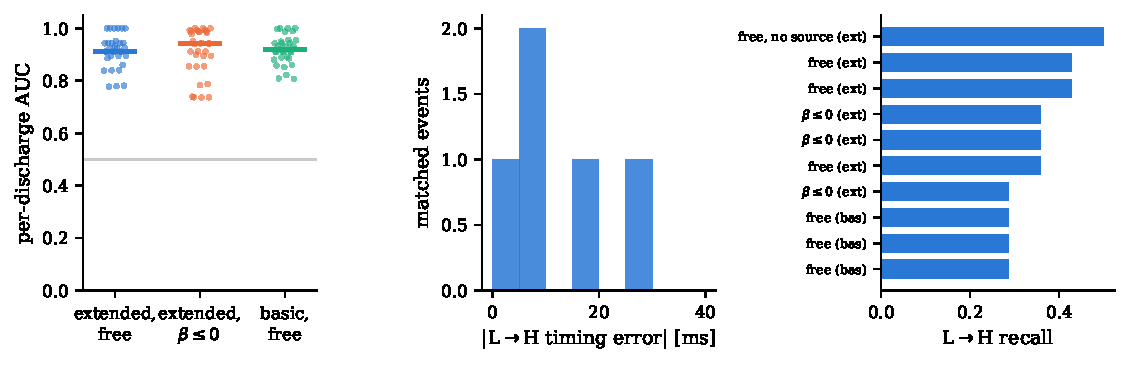
\includegraphics[width=\linewidth]{figures/fig_aggregate}
  \caption{Aggregate held-out performance. Left: per-discharge AUC for the
  three configurations, all seeds pooled, with medians marked; the chance
  level is indicated. Centre: distribution of matched L$\to$H timing
  errors. Right: L$\to$H recall by configuration. The overlap of the AUC
  distributions between the free and constrained-monostable arms is the
  visual form of the null result discussed in the text.}
  \label{fig:aggregate}
\end{figure}

\begin{table}[t]
\centering\small
\caption{Model comparison on grouped validation. All rows share data,
splits, solver, optimiser, stopping rule, and parameter budget; only the
named factor differs. $r_{\mathrm{LH}}$ is L$\to$H event recall,
H-basin the fraction of discharges in which the latent reaches the upper
branch. Generated by \texttt{scripts/final\_report.py}.}
\label{tab:comparison}
\begin{tabular}{llrrrrrrr}
\toprule
drive & latent & val loss & AUC & F1 & Brier & $r_{\mathrm{LH}}$ & $\beta$ & H-basin \\
\midrule
extended & $\beta\leq 0$ (s2) & 0.461 & 0.948 & 0.00 & 0.156 & 0.10 & -0.78 & 0.98 \\
\bottomrule
\end{tabular}
\end{table}

\subsection{Fold margins and conditional thresholds}
\label{sec:res-folds}

Because the topology question is not decided (\S\ref{sec:res-modelcomp}),
the fold quantities below characterise the free-topology fit; they are not
offered as established properties of the experiment. For that fit
$\beta = \resBeta$ with a seed spread of $\pm 0.004$, giving folds at
$\dr_{\mathrm{f}}^{\pm} = \pm\resFoldHigh$ and a latent time scale
$\tau = \resTau\,$ms, consistent with the observed few-tens-of-ms
transition duration. Converting the upper fold to an equivalent
injected-power threshold requires holding all other covariates fixed and
dividing by the power coefficient; the result is a conditional slice of a
threshold surface, not a universal threshold, and it is not comparable in
absolute value to published loss-power thresholds for the reasons given in
Appendix~\ref{app:data-limits}.

\begin{figure}[t]
  \centering
  
\includegraphics[width=0.56\linewidth]{figures/fig_bifurcation}
  \caption{Equilibrium manifold of the identified free-topology latent
  (solid: stable branches; dashed: saddle) with the inferred trajectory
  $\big(\dr(\inr(t)), \lat(t)\big)$ of one held-out discharge
  overlaid, coloured by time. This characterises the fitted parameter set;
  \S\ref{sec:res-modelcomp} explains why it is not evidence that the data
  require folds.}
  \label{fig:bifurcation}
\end{figure}

\begin{figure}[t]
  \centering
  
\includegraphics[width=0.66\linewidth]{figures/fig_margins}
  \caption{Static fold margins \eqref{eq:margins} along a held-out
  discharge for the free-topology fit. $\mLH$ reaching zero marks the
  disappearance of the quasi-static low-confinement equilibrium, which
  under a finite-rate drive precedes the observed transition by a dynamic
  delay.}
  \label{fig:margins}
\end{figure}

\begin{figure}[t]
  \centering
  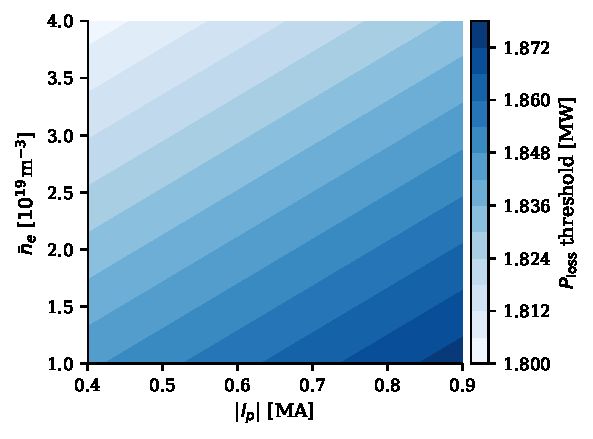
\includegraphics[width=0.5\linewidth]{figures/fig_threshold}
  \caption{Conditional equivalent-power threshold surface implied by the
  identified drive, as a function of plasma current and density with the
  remaining covariates held fixed. A single threshold number is one slice
  of this surface; the absolute values are corpus-specific and are not
  comparable to published loss-power thresholds
  (Appendix~\ref{app:data-limits}).}
  \label{fig:threshold}
\end{figure}

\subsection{Runtime and streaming replay}
\label{sec:res-runtime}

The deployed quantities are a single scalar ODE step and two closed-form
readouts. Replaying the identified latent causally over held-out
discharges, using only past and current inputs and no D$_\alpha$, costs a
few microseconds per step in a plain NumPy implementation representative of
a plasma-control-system environment, against a $\SI{1}{ms}$ actuator
cadence. The profile solve is not required for the regime estimate. We
therefore describe the regime assessor as control-oriented and explicitly
not control-ready: there is no observer correcting drift, no closed-loop
test, and the H$\to$L behaviour documented in \S\ref{sec:res-events}
would need to be resolved first.

\subsection{Locked-test evaluation}
\label{sec:res-test}

% Written after the single evaluation on the held-out sessions.
\emph{TODO: single-pass locked-test numbers.}
